\documentclass[UTF8]{ctexart}
\usepackage[left=3.2cm,right=3.2cm,top=2.33cm,bottom=2.33cm]{geometry}
\usepackage{fancyhdr}
\usepackage{graphicx}
\pagestyle{fancy} 
\rhead{\sf Machine Learning}		% 标题
\cfoot{\thepage}
\rfoot{\color{gray}\tt Linear Model}
\usepackage[svgnames]{xcolor}
\usepackage{hyperref}
\setlength\parskip{.3\baselineskip}
\hypersetup{
	%   bookmarks=true,     	% show bookmarks bar?
	%   CJKbookmarks=true,     	% 中文支持
	unicode=true,          	% non-Latin characters in Acrobat’s bookmarks
	pdftoolbar=true,        	% show Acrobat’s toolbar?
	pdfmenubar=true,        	% show Acrobat’s menu?
	pdffitwindow=false,     	% window fit to page when opened
	pdfstartview={FitH},    	% fits the width of the page to the window
	%pdftitle={My title},    % title
	%pdfauthor={Author},     % author
	%pdfsubject={Subject},   % subject of the document
	%pdfcreator={Creator},   % creator of the document
	%pdfproducer={Producer}, % producer of the document
	%pdfkeywords={keywords}, % list of keywords
	%pdfnewwindow=true,      % links in new window
	colorlinks=true,         % false: boxed links; true: colored links
	linkcolor=Black,		  	% color of internal links
	citecolor=Magenta,      	% color of links to bibliography
	filecolor=green,        	% color of file links
	urlcolor=DarkBlue       	% color of external links
}
\usepackage{enumerate}
\usepackage{amssymb, amsmath, mathrsfs, mathtools}
\usepackage{amsthm}
\usepackage{listings}
\lstset{
	numbers = left, % 想要代码行号请反注释这一行
	numberstyle = \small\ttfamily,
	frame = shadowbox,
	basicstyle = \ttfamily \bfseries,
	keywordstyle = \color{blue!70},
	commentstyle = \color{red!50!green!50!blue!50}, 
	rulesepcolor= \color{red!20!green!20!blue!20},
	xleftmargin = 0.3em,
	xrightmargin = 0.5em,
	% aboveskip = 1em
} 
% \lstset{numbers=left, frame=shadowbox, basicstyle=\ttfamily, commentstyle=\fontseries{lc}\selectfont\slshape, columns=fullflexible, breaklines=true, escapeinside={(*@}{@*)}} % From LM
\newtheorem{lemma}{引理}
\begin{document}
	\begin{titlepage}
		\vspace*{\fill}
		\begin{center}
			\normalfont
			{\Huge \bfseries 机器学习上机报告}
			
			\bigskip
			
			{\Large \itshape 林远钊 1700010672}
			
			\medskip
			
			\today
		\end{center}
		\vspace{\stretch{3}}
	\end{titlepage}
	\newpage
	\tableofcontents
	
	\newpage
\section{线性模型Linear Model}
本次上机作业中主要涉及到两个线性模型:Logistic回归模型(西瓜书中译为对数几率回归模型)和线性判别分析模型(Linear Discriminant Analysis)。

\subsection{Logistic回归}
尽管名字中带有回归二字,实际上这仍是一个分类器。在文献中还被称为Logit回归、最大熵分类和对数线性分类器。

严格的说,西瓜书上具体介绍的对数几率回归应当属于是二项Logistic回归模型(之后才拓展为多分类模型),思想主要是通过Logistic函数$ \frac{1}{1+e^{\omega x +b}} $,衍生出对对数几率$ ln(\frac{y}{1-y}) $的定义,并对其进行极大似然估计

\subsection{线性判别分析}
线性判别分析的思想也比较朴素,给定样本数据集,试图将样例投影到一条直线上,使得:
\begin{enumerate}[i]
	\item 同类样例点投影尽可能接近
	\item 异类样例点投影尽可能远离
\end{enumerate}
并且在新样例点分类问题中,以其投影点所在的位置来确定新样本的类别。

最终形式化的最大化目标便根据以上的朴素思想定义为异类样例中心的距离和同类样例投影点的协方差的比值,通过奇异值分解而保证数值解的稳定后,可以得到最终模型所需直线的$ \omega $值
\section{工具介绍}
\subsection{对数几率回归}
此处介绍科学计算包sklearn当中支持的关于Logistic回归(对数几率回归)的类。可以通过命令导入类sklearn.linear\_model.LogisticRegression。这个类实现了正则化的Logistic回归,支持二分类和多分类问题(采用OvR策略)或者多项式正则回归(通过参数L1,L2采取不同的模式)。使用了'liblinear'库,有"newton-cg","sag"和"lbfgs"三种得到最优化问题最优解的求解程序。

核心求解程序中,'lbfgs','sag'和'newton-cg'只支持L2型的优化问题,在实践中发现它们对一些高维数据收敛得很快。其中'sag'代表的是随机梯度下降法(Stochastic Average Gradient descent),对于大的数据集(特征数和样本数都很大的时候),它比其余几种算法都要快;'lbfgs'是一个和 Broyden-Fletcher-Goldfarb-Shanno算法(是拟牛顿方法的一种)近似的最优化算法,该算法适用于小数据集,而它在大数据集中的表现比较糟糕。

另外,在完成3.4题中,需要使用交叉验证法来评估习得模型的性能,交叉验证法的代码实现并不复杂,此处便直接使用LogisticRegressionCV包来完成此处的任务。使用和LogisticRegression类基本一致,唯一需要注意的参数是控制折数的cv。
\subsection{线性判别分析}
可以通过命令from sklearn.discriminant\_analysis import LinearDiscriminantAnalysis导入sklearn中用于线性判别分析(LDA)的类,是一个分类器。使用的模式基本和之前用到的classifiers相似(大概是python中的magic method理念)。

这种分类器的优点在于容易计算实现,而且这种方法在实际应用中被证实是有效的,同时这种方式也无过多调参的负担。问题当然就是——只能学习线性边界的问题。

\section{实现概述}
首先解决3.3和3.4中关于对数几率回归的问题,鉴于UCI数据集的数据更为充分,为了更好体现学习的效果和过程,首先以iris数据集和wine数据集为例给出实现代码。
\begin{figure}[htbp]
	\centering
	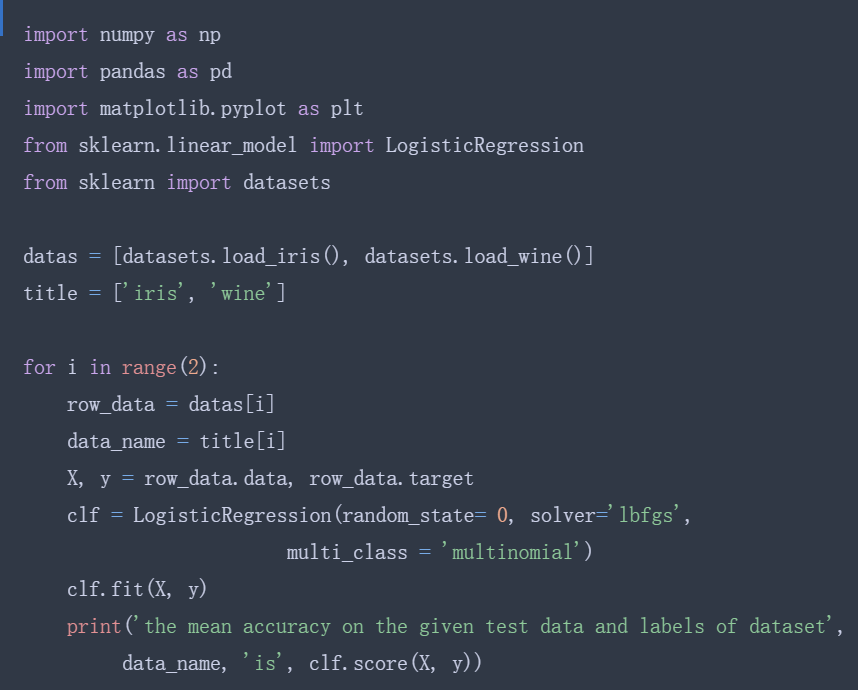
\includegraphics[scale=0.7]{row.PNG}
	\caption{row\_data}
\end{figure}

以上直接对iris和wine数据集进行了logistic回归,并且输出了习得模型在原有数据的准确度均值如下
\begin{figure}[htbp]
	\centering
	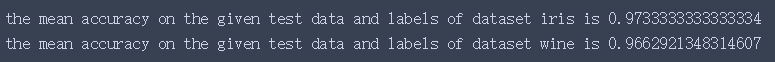
\includegraphics[scale=0.8]{row_ans.PNG}
	\caption{row\_ans}
\end{figure}

大致熟悉了使用方法后,就可以将之应用在西瓜数据集3.0alpha上,实现代码和之前类似
\begin{lstlisting}[language=python]
def loadData(filename):
	"""默认csv文件第一行是列属性,以下每行是训练数据
	并且数据的最后一列必然是数据的label"""
	frame = pd.read_csv(filename)#读为DataFrame格式
	labels = frame['label']#获取标记
	attrset = list(frame.columns)
	attrset.remove('label')
	dataset = list(frame.values)
	for i in range(frame.shape[0]):#遍历所有数据
		dataset[i] = list(dataset[i])
	dataset[i].pop()
	return dataset, list(labels), attrset
	
X, y, labels = loadData("data3.0alpha.csv")
clf = LogisticRegression(random_state= 0, solver='lbfgs', 
	multi_class = 'multinomial')
clf.fit(X, y)
clf.score(X,y)
\end{lstlisting}

此时的输出结果是0.7058823529411765,在习得模型对原数据的预测性能明显下降,原因大约来自于两个方面
\begin{enumerate}
	\item 西瓜数据集中样本量太少
	\item 西瓜数据集3.0$ \alpha $中含糖率和密度关于好瓜坏瓜的分类问题不是线性的(这个其实从上一次SVM作业中的高斯核和线性核学习能力比较也可看出)
\end{enumerate}

另一方面,也可以在开始试验的基础上使用LogisticRegressionCV进行十折交叉验证。
\begin{lstlisting}[language = python]
from sklearn.linear_model import LogisticRegressionCV
#交叉验证的函数实现起来也并不复杂,这里直接调用现成的包
for i in range(2):
	row_data = datas[i]
	data_name = title[i]
	X, y = row_data.data, row_data.target
	clf = LogisticRegressionCV(cv = 10, random_state=0,
		max_iter=1000,solver = 'lbfgs',
		multi_class = 'multinomial')
	clf.fit(X, y)
	print('the mean accuracy using 10-folds cross validation',      
		data_name, 'is', clf.score(X,y))  
\end{lstlisting}

这里要注意,在设定分类器的时候,笔者对最大迭代次数max\_iter进行了设定——如果采用默认方案会报收敛性错误(ConvergenceWarning)。最终两个数据的评估结果分别是0.9866666666666667和0.9775280898876404,可以看到模型学习性能有一定提升。

类似的可以给出留一法的实现,留一法实际就相当于折数等于样本数。这里为了适应sklearn包的特点,调用from sklearn.model\_selection import LeaveOneOut,并令参数cv等于LeaveOneOut(),最终训练得到iris数据集结果是0.98,wine数据集由于数据量比较大采用LeaveOneOut迭代耗时较长,最终评分甚至达到了1.00.

之后是3.5题中的线性判别分析问题,核心实现其实大同小异,这里不再赘述(其实是用Jupyter notebook 写完后没保存qwq),此题中笔者还给出了问题的可视化学习结果,其中点代表样本点,叉代表了那一类样本的均值点。
\begin{figure}[htbp]
	\centering
	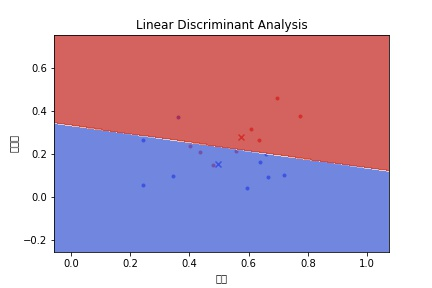
\includegraphics[scale=0.8]{LDA.jpg}
	\caption{LDA}
\end{figure}

其中横轴是密度,纵轴是含糖率(由于代码丢失,我在使用图片时才发现出现了不支持中文的问题,但是画图实在实在实在太麻烦了qwq就没有再写一遍,在此说明,请助教老师见谅)

(ps:附件中包含所有源码和用到的图片,源码由于部分使用jupyter notebook笔记本的方式,其中代码可能有些乱)
\end{document}
